The majority of accounts of local markers tend to focus on the development of the Bott index and the Chern marker. However, the first construction of a real-space Chern number can, along with the rest of modern physics, be found in the appendices of a seminal work by Kitaev \cite{kitaev_anyons_2006}. Thus, we shall start our discussion with an explanation of Kitaev's local marker, the discussion will largely follow the source material, however we provide some detail at various points where it is brushed passed there. 

\begin{figure}
    \centering
     \begin{center}
        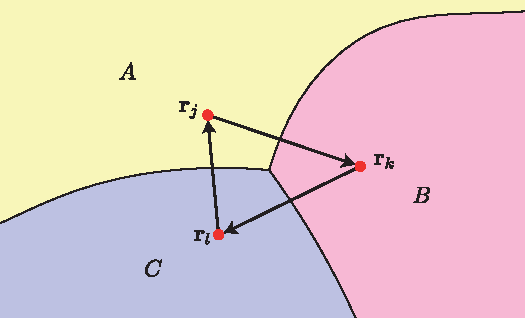
\includegraphics[]{local_markers/figures/h_jkl.pdf}
    \end{center}
     \captionof{figure}{
     Diagram showing the partition of the plane into three regions labelled with $A$, $B$ and $C$. An example of $h_{jkl}$ is depicted with red dots, where arrows indicate the positive direction. 
     }\label{fig:h_jkl}
\end{figure}
 
As always, our starting point is a Hamiltonian defined on an arbitrary lattice with sites at positions $\textbf r_j$, however in this case we shall work in the case of a system with infinite boundary conditions. Here, let us define the projector onto a band $P = \sum_{\textup{band}} \ketbra{\psi}{\psi}$, along with a shorthand for off-diagonal correlations given by 
\begin{align}
    P_{jk} = \braket{\textbf r_j |P| \textbf r_k}.
\end{align}
In general, if this is onto a gapped set of states, then the projector will have exponentially localised correlations \cite{hastings_spectral_2006},
\begin{align}
    |P_{jk}| \leq c|\textbf r_j - \textbf r_k|^{-\alpha}
\end{align}
\begin{shaded}
    maybe add an argument for why this has to be the case -- see the Paley-Wiener theorem
\end{shaded}
Following Kitaev, let us define a 2-current,
\begin{align}
    h_{jkl} = 12\pi i (P_{jk}P_{kl}P_{lj} - P_{jl}P_{lk}P_{kj}).
\end{align}
We divide our system into three regions in real space, $A$, $B$ and $C$, and define the real-space Chern number,
\begin{align}
    \qkit(P) = \sum_{j \in A}\sum_{k \in B}\sum_{l \in C} h_{jkl},
\end{align}
which we can re-express in terms of a set of projectors onto the three regions,
\begin{align}
    \qkit(P) = 12\pi i \tr( PAPBPC - PCPBPA) .
\end{align}
This quantity remains invariant when we relabel any finite area from one region to another. 

\begin{shaded}
    {\it The Invariance of $\qkit$ to changes in $A$, $B$ and $C$ --- } In order to see why this is the case, let us consider picking up some finite chunk of the region $B$, which we label with $\alpha$ and moving it over into region $A$. Thus, let us make the redefinition
    \begin{align}
        A' &= A + \alpha \\
        B' & = B - \alpha
    \end{align}
    \begin{center}
        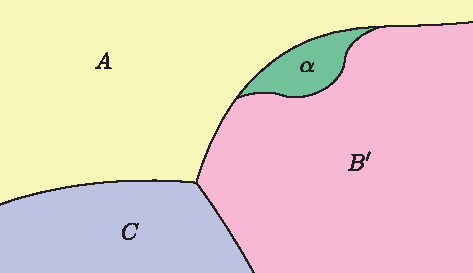
\includegraphics[]{local_markers/figures/alpha_region.pdf}
    \end{center}
    Thus, the matrix term in the Kitaev Chern number becomes
    \begin{align}
        PAPBPC - h.c. = PA'PB'PC 
        + PAP\alpha PC 
        - P\alpha PB'PC - h.c.
    \end{align}
    Now let us use the identity $B' = \1 - \alpha - A - C$ to re-express this in the form
    \begin{align}\begin{split}
        PAPBPC - h.c. = & PA'PB'PC 
        + PAP \alpha P C
        + P\alpha PAPC \\ 
        & - P\alpha PC
        + P\alpha P\alpha PC
        + P\alpha PCPC  - h.c.
    \end{split}
    \end{align}
where we have used the identity $P^2 = P$ to obtain this line. All the extra terms on the RHS vanish when the trace is taken. Note that generally one cannot use the cyclic property of the trace here, since our operators are infinite matrices, so there is no guarantee that the rearranged infinite sum converges to the same value. However, since $\alpha$ represents a finite region, the sum vanishes far from $\alpha$ and so we are free to cycle any trace containing $\alpha$. Thus we are left with
\begin{align}\begin{split}
    \tr (PAPBPC - h.c.) = \tr (PA'PB'PC  - h.c.).
\end{split}
\end{align}
In fact, the extra finite region $\alpha$ need not be a projector, since the above proof holds regardless of the properties of $\alpha$ provided that it has finite support. Thus we can go even further and see that the value of $\qkit$ is invariant under the addition of any finite matrix to one region, provided we subtract it from another region as well.


\end{shaded}  

Let us re-express $\qkit$ to a form that will be useful in the following discussion. Since the expression is invariant under cycling of the order of our three regions, we may write it as
\begin{align}
    \qkit = 4 \pi i \tr(
        &PAPBPC + PBPCPA + PCPAPB \\
        &- PAPCPB - PCPBPA - PBPAPC),
\end{align}
note that we are not allowed to cycle the terms in the trace here. Inserting the identity 
\begin{align}\label{eqn:cab_identity}
    C = \1 - A - B,
\end{align} 
we arrive at the following expression,
\begin{align}
    \qkit(P) = 4 \pi i \tr[
        PAP, PBP
    ]
\end{align}
This is a trace of a commutator, which will always vanish if one of the operators in the commutator has finite support. This supports our assertion that $\qkit$ is invariant under addition of any finite matrix to $A \rightarrow A + \alpha$, since $\tr[P\alpha P, PBP]$ vanishes. Of course we must also transform either $B \rightarrow B-\alpha$ or $C \rightarrow C-\alpha$ for the identity \ref{eqn:cab_identity} to hold.

This invariance to the form of $A, B$ and $C$ affords us with an astounding amount of freedom in how we choose to define this Chern number. Not only can we select any three regions with any shape (provided the overall topology of the three regions far from the triple contact point remains the same). We can even blur the boundaries between the projectors or allow them to overlap and nothing will change.

\subsection{Relation to the Chern Number}

So far we have constructed a quantity, $\qkit$ and shown that there is a remarkable amount of freedom in how we can build it without changing the value. In order to connect this to band topology, we will need to show that when evaluated in a translationally symmetric context, $\qkit$ corresponds exactly to the Chern number. Let us start by re-expressing $\qkit$ again in a new form. We define a set of step function projectors $\vartheta_x, \vartheta_y$ that satisfy 
\begin{align}
    \vartheta_\alpha \ket{\textbf r} = 
    \begin{cases}
        \ket {\textbf r}&\textup{ for }r_{\alpha} \geq 0,\\ 
        0&\textup{ for }r_{\alpha} < 0.
    \end{cases}
\end{align} 
Let us now consider the operator
\begin{align}
    2 \pi i \tr
    [ P\vartheta_x P, P\vartheta_y P ].
\end{align}
\begin{center}
        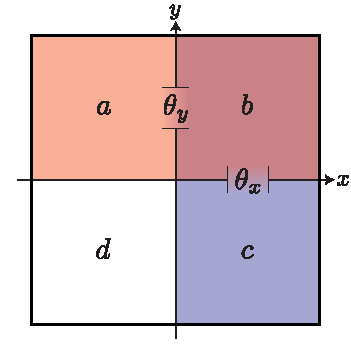
\includegraphics[]{local_markers/figures/four_boxes.pdf}
\end{center}
By decomposing the step function into projectors onto the four quarters of the plane, we arrive at
\begin{align}\begin{split}
    2\pi i\tr [P \vartheta_xP, P \vartheta_yP ] = 2\pi i \tr \big ( 
        &[P a P, P b P ] + 
        [P b P, P b P ] \\
        &+[P a P, P c P ] 
        +[P b P, P c P ]
        \big )    
\end{split}
\end{align}
Clearly the second term on the RHS vanishes. The third term also vanishes, which can be seen by its invariance under a mirror symmetry across the line $y +x = 0$ (a mirror reflection will always change the sign of $h_{jkl}$). Finally, we see that the first and last terms are both equal to $\qkit/2$, thus
\begin{align}
    \qkit = 2\pi i\tr [P \vartheta_xP, P \vartheta_yP ].
\end{align}
In order to make contact with momentum space, we shall work in an infinite translational system. Clearly, in this context the position of the step functions will have no effect on the value of $\qkit$. Thus, let us define a set of translated step functions
\begin{align}
    \vartheta_\alpha(\textbf R) \ket{\textbf r} = 
    \begin{cases}
        \ket {\textbf r}&\textup{ for }r_{\alpha} \geq R_\alpha,\\ 
        0&\textup{ for }r_{\alpha} < R_\alpha.
    \end{cases}
\end{align} 
Obviously, the value of $\qkit(\textbf R) = 2\pi i\tr [P \vartheta_x(\textbf R) P, P \vartheta_y(\textbf R)P ]$ is constant. Thus let us choose some square region of area $L^2$ the plane and take the average of $\qkit(\textbf R)$ over this region, 
\begin{align}
    \qkit &= \frac{1}{L^2} \int_{-L/2}^{L/2} dR_x\, dR_y\, \qkit(\textbf R)  \\ 
    & = \frac{2\pi i}{L^2} \tr [ PxP, PyP ] \\ 
    & = \frac{2\pi i}{L^2} \tr P \big[ [x,P],[y,P] \big ] 
\end{align}
In the limit of large L, we expect that the contribution to the trace is uniform in space, and so can replace the global trace with a local trace around some arbitrary point in the system $\textbf r$, $\frac1 {L^2} \tr \rightarrow \loctr_{\textbf{r}} $. Thus we arrive at 
\begin{align}
    \qkit = 2\pi i \loctr _{\textbf{r}} \big [P[x,P],[y,P]\big ]. 
\end{align}
Now let us construct the exact form of the projector onto a band for a translationally symmetric Hamiltonian. From Bloch's theorem, we know the projector will have the following form
\begin{align}
    P = \frac{1}{4\pi^2}\int d^2 \textbf k \ketbra k k \otimes \psi(\textbf k)
\end{align}
This means that we can use the identity $[x, P] \rightarrow -i \partial_x \psi(\textbf k)$ to show that 
\begin{align}
    \qkit = \frac{-i}{2\pi} \int d^2 \textbf k \, 
    \loctr _{\textbf{r}} \big (\ketbra {\textbf k} {\textbf k} \otimes
        \psi(\textbf k) [\partial_x \psi(\textbf k), \partial_y \psi(\textbf k)]
    \big )
\end{align}
Now, using the fact that $ \braket{\textbf r \ketbra{\textbf k}{\textbf k}  \textbf r}  = 1$, this reduces to a trace over the unit cell degree of freedom only,
\begin{align}
    \qkit = \frac{-i}{2\pi} \int d^2 \textbf k \, 
    \tr \big (
        \psi(\textbf k) [\partial_x \psi(\textbf k), \partial_y \psi(\textbf k)]
    \big ).
\end{align} 
Comparing to eqn.~\ref{eqn:operator_berry_curvature}, we see that this quantity exactly evaluates an integral of the Berry curvature over the Brillouin zone. Thus we have shown that -- at least in the context of an infinite, translationally symmetric system -- $\qkit$ evaluates the Chern number.

\begin{shaded}
    {\it A Useful Identity for Operators in Momentum Space --- } Let us start by considering an arbitrary operator in a translationally symmetric system with the following form,
    \begin{align}
        A =  \int_{BZ} \frac{d k}{2\pi} \ketbra k k \otimes A(k),
    \end{align}
    where $A(k)$ acts on the degrees of freedom inside the unit cell. Here we use a 1D Brillouin zone, but this can be straightforwardly extended to 
    higher dimensions. Let us consider the following expression,
    \begin{align}
        [x, A] = \frac{1}{2\pi} \int_{BZ} d k \big [x,\ketbra k k \big ] \otimes A(k).
    \end{align} 
    using the identity $x\ket k = i\partial_k \ket k$, we can rewrite this in the form
    \begin{align}
        [x, A] & = \frac{1}{2\pi} \int_{BZ} d k\, i \partial_k \big(\ketbra k k \big) \otimes A(k) \\ 
        &= \frac{1}{2\pi} \int_{BZ} d k\,  \ketbra k k 
        \otimes ( -i \partial_k A(k)),
    \end{align} 
    where we used the fact that an integral of total derivative of the RHS vanishes, as the integral is over the whole Brillouin zone. Thus, we can make the general substitution
    \begin{align}
        [x,A] \rightarrow -i \partial_{k} A(k)
    \end{align}
\end{shaded}

\subsection{Kitaev's Marker in a Finite System}

So far, we have defined Kitaev's chern number for a system with infinite boundary conditions. This version of the Chern number is useful in analytical arguments -- for example, such a Chern number was used to prove the quantisation of Hall conductivity in the presence of disorder \cite{bellissard_noncommutative_1994}. However, to be of practical use, $\qkit$ must still work in a 


